\subsubsection{Problém rozkladu na sčítance}
\label{sssec:problem-rozkladu-na-scitance}

Oblíbený problém, který lze řešit počítáním způsobů, jak volit počet sourodých
předmětů z většího množství, ale nikdo by to na první pohled nečekal, je
\emph{problém rozkladu na sčítance}.

Volme číslo $m \in \N$. \emph{Rozkladem čísla $m$ na $r$ sčítanců} myslíme
rovnost
\[
 m = x_1 + x_2 + \cdots + x_r = \sum_{k=1}^{r} x_k,
\]
kde $x_i \geq 0$ jsou nezáporná celá čísla. Zajímá nás, kolika způsoby lze dané
číslo $m$ rozložit na $r$ (ne nutně různých) sčítanců. Na první pohled nejde
vůbec o kombinace (tedy o výběr bez závislosti na pořadí), protože pořadí
sčítanců je zde důležité: rozklad $7 = 0 + 2 + 5$ \textbf{je různý} od rozkladu
$7 = 2 + 0 + 5$. Situace se navíc v tomto směru zdá zcela beznadějná, neboť když
jsou dvě a více čísel v rozkladu stejná, pak jejich prohození samozřejmě
neurčuje jiný rozklad. Například, v rozkladu $7 = 2 + 2 + 3$ mohu prohodit první
$2$ s druhou $2$ a nedostat tak odlišný rozklad.

První průlomovou myšlenkou je náhled, že číslo $m$ vlastně \uv{rozhazuji} mezi
$r$ čísel. V tomto smyslu si lze představit přirozené číslo $m$ jako $m$
nerozlišitelných míčků, které rozděluji do $r$ košíků. Třeba rozklad $7 = 0 + 2
+ 5$ by vypadal takto.

\begin{figure}[h]
 \centering
 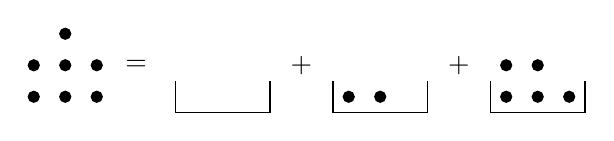
\begin{tikzpicture}
  \foreach \i in {-0.4,0} {
   \foreach \j in {0,0.4,0.8} {
    \draw[fill=black]  (\j, \i) circle (2pt);
   }
  }
  \draw[fill=black] (0.4, 0.4) circle (2pt);

  \node at (1.3, 0) {$=$};

  \foreach \j in {0,0.4} {
   \draw[fill=black]  (4 + \j, -0.4) circle (2pt);
  }

  \draw (1.8, -0.2) -- (1.8,-0.6);
  \draw (1.8, -0.6) -- (3,-0.6);
  \draw (3, -0.6) -- (3,-0.2);

  \node at (3.4,0) {$+$};

  \draw (3.8, -0.2) -- (3.8,-0.6);
  \draw (3.8, -0.6) -- (5,-0.6);
  \draw (5, -0.6) -- (5,-0.2);

  \node at (5.4,0) {$+$};

  \foreach \j in {0,0.4,0.8} {
   \draw[fill=black]  (6 + \j, -0.4) circle (2pt);
  }
  \draw[fill=black]  (6, 0) circle (2pt);
  \draw[fill=black]  (6.4, 0) circle (2pt);

  \draw (5.8, -0.2) -- (5.8,-0.6);
  \draw (5.8, -0.6) -- (7,-0.6);
  \draw (7, -0.6) -- (7,-0.2);
 \end{tikzpicture}
 \label{fig:micky-do-kosiku}
 \caption{Vizualizace rozkladu $7 = 0 + 2 + 5$ jako rozdělení míčků do košíků.}
\end{figure}

Samozřejmě, v takovémto rozkladu určuje pravá strana jednoznačně tu levou, takže
není třeba $7$ míčků na levé straně znázorňovat. Podobně, když se dohodneme, že
počty míčků v košících vždy sčítáme, lze i symboly $+$ vynechat. Trochu
složitější rozklad, třeba $9 = 1 + 0 + 3 + 5$ bychom nakreslili jak vidno na
\hyperref[fig:jenom-micky-a-kosiky]{obrázku~\ref*{fig:jenom-micky-a-kosiky}}.

\begin{figure}[h]
 \centering
 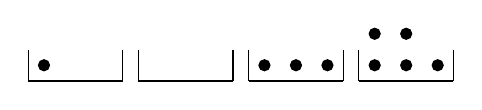
\begin{tikzpicture}
  \foreach \k in {0} {
   \draw (\k,-0.2) -- (\k,-0.6);
   \draw (\k,-0.6) -- (\k+1.2,-0.6);
   \draw (\k+1.2,-0.6) -- (\k+1.2,-0.2);
  }
  \draw[fill=black]  (0.2, -0.4) circle (2pt);

  \foreach \k in {1.4} {
   \draw (\k,-0.2) -- (\k,-0.6);
   \draw (\k,-0.6) -- (\k+1.2,-0.6);
   \draw (\k+1.2,-0.6) -- (\k+1.2,-0.2);
  }

  \foreach \k in {2.8} {
   \draw (\k,-0.2) -- (\k,-0.6);
   \draw (\k,-0.6) -- (\k+1.2,-0.6);
   \draw (\k+1.2,-0.6) -- (\k+1.2,-0.2);
  }
  \foreach \j in {0,0.4,0.8} {
   \draw[fill=black]  (3 + \j, -0.4) circle (2pt);
  }

  \foreach \k in {4.2} {
   \draw (\k,-0.2) -- (\k,-0.6);
   \draw (\k,-0.6) -- (\k+1.2,-0.6);
   \draw (\k+1.2,-0.6) -- (\k+1.2,-0.2);
  }
  \foreach \j in {0,0.4,0.8} {
   \draw[fill=black]  (4.4 + \j, -0.4) circle (2pt);
  }
  \foreach \j in {0,0.4} {
   \draw[fill=black]  (4.4 + \j, 0) circle (2pt);
  }
 \end{tikzpicture}
 \caption{Zjednodušený nákres rozdělení míčků do košíků.}
 \label{fig:jenom-micky-a-kosiky}
\end{figure}

Nakonec si uvědomíme, že přeci není ani třeba kreslit jednotlivé košíky. Stačí,
když všechny míčky vysypeme na zem a jenom mezi ně dáme nějaká hradla, abychom
věděli, které míčky patřily do stejného košíku. Názorná ukázka, pro stejný
rozklad, tedy $9 = 1 + 0 + 3 + 5$.

\begin{figure}[h]
 \centering
 
\begin{tikzpicture}
  \draw[fill=black] (0, 0) circle (2pt);
  \draw[thick] (0.5, 0.2) -- (0.5, -0.2);
  \draw[thick] (1, 0.2) -- (1, -0.2);
  
  \foreach \i in {0,0.3,0.6} {
   \draw[fill=black] (1.5 + \i, 0) circle (2pt);
  }

  \draw[thick] (2.6, 0.2) -- (2.6, -0.2);
  \foreach \i in {0,0.3,...,1.5} {
   \draw[fill=black] (3.1 + \i, 0) circle (2pt);
  }
 \end{tikzpicture}
 \caption{Ještě jednodušší nákres rozkladu $9 = 1 + 0 + 3 + 5$.}
 \label{fig:nejjednodussi-micky-s-kosiky}
\end{figure}

Jeden možný způsob, jak si snadno představit spojitost mezi rozkladem a touto
poslední verzí jeho vizualizace je ten, že stěny či hradla odpovídají symbolům
$+$ a počet míčku mezi dvěma hradly odpovídá číslu mezi příslušnými symboly.
Protože sčítanců je $r$, a tedy symbolů $+$ je $r - 1$, je hradel též $r - 1$.

Jsme připraveni řešení úlohy završit. Rozmysleli jsme si, že každé rozmístění $r
- 1$ hradel mezi $m$ za sebou v řadě ležících míčků mi definuje jeden konkrétní
rozklad čísla $m$ na $r$ sčítanců. Stačí tedy umět určit počet takových
rozmístění.

To ale není těžké. Míčky a hradla činí dohromady $m + r - 1$ objektů, z kterých
přesně $r - 1$ jsou hradla. Řečeno jinak, když z $m + r - 1$ objektů vyberu těch
$r - 1$, která se stanou hradly, a zbytek přetvořím v míčky, pak určím rozklad
čísla $m$ na $r$ sčítanců. Počet všech možných výběrů $r - 1$ prvků z~množiny o
$m + r - 1$ prvcích je $\binom{m + r - 1}{r-1}$, kteréžto číslo je tudíž i počet
způsobů, jak rozložit číslo $m$ na $r$ sčítanců.
